\documentclass[11pt, oneside]{article}   	% use "amsart" instead of "article" for AMSLaTeX format
\usepackage{geometry}                		% See geometry.pdf to learn the layout options. There are lots.
\geometry{letterpaper}                   		% ... or a4paper or a5paper or ... 
%\geometry{landscape}                		% Activate for rotated page geometry
%\usepackage[parfill]{parskip}    		% Activate to begin paragraphs with an empty line rather than an indent
\usepackage{graphicx}				% Use pdf, png, jpg, or eps§ with pdflatex; use eps in DVI mode
								% TeX will automatically convert eps --> pdf in pdflatex	
\usepackage{caption}
\usepackage{subcaption}
\usepackage{float}

\graphicspath{ {./LabReportAssignment1Images/}}	
\usepackage{amssymb}

%SetFonts

%SetFonts


\title{Assignment 1: \\ Per-night price prediction with AirBnB}
\author{\centering Ivo L. Arasin (r0926378) \and Vancesca Dinh (r0930510) \and Linas J. Leščinskas (r0874301) \and Yavuz Yavuzhan (r0920104)}
%\date{}							% Activate to display a given date or no date

\begin{document}
\maketitle
\section{Exploratory Data Analysis}
\indent The aim of this report is to detail the approach our group has taken in an effort to build a predictive model for per-night prices of AirBnB listings. The dataset at hand contains 6495 listings along 55 features. Many of the features are not readily usable in a model. Initial exploratory data analysis revealed that, at least up front, no variable has any explanatory power with respect to the target (c.f. Figure 1). 34 features have missing values, although this is counting all features that have at least one observation missing. Still, 21 features have more than 10\% missing values. The worst offender is \textit{property\_sqfeet} with $>$97\% missing values. Many of the missing values, especially in the reviews-category coincide (c.f. Figure 2). Additionally, there are many textual features that would require transformation to be useful. There are no duplicate rows. \newline
\indent In what follows, we detail the steps taken to preprocess and manipulate the data to distill as much predictive power as possible. 
\section{Data Cleaning \& Feature Engineering}

\subsection{Numerical features and geolocation}
\textit{property\_sqfeet}, despite its many missing values, might hold some information. A closer look reveals grave inconsistencies in the observations that do exist, i.e. sometimes the values indicate square-feet, other times square-meters. Visual inspection of square-feet and target-price reveals a good threshold to differentiate between the two metrics is 150 (based on trial and error and the intuition that there are no listings offering a room with a size of $<14m^2$). Accordingly, all listings with \textit{property\_sqfeet} $<$ 150 are multiplied with the conversion factor 10.764 to convert $m^2$ to $feet^2$.  Missing values were replaced with zeros. When filtering out all zero-values, \textit{property\_sqfeet} now has a correlation with the target of $\sim$23\%, as opposed to the $\sim$15\% before.\newline
\newline
\indent Missing \textit{property\_zipcode} values are imputed based on k-nearest-neighbours with n=4. Then, the \textit{property\_zipcode} column is replaced with two new columns. One is indicating the frequency of occurrence, the other mean-encodes the target per zipcode, i.e. for every zipcode-group the target-mean is computed based on the training-data. If the test-data contains previously unseen zipcodes, the column makes use of the overall target-mean computed based on the training-set.\newline
\newline
\indent Numerical features with missing values are imputed with a linear regression whose independent variables were picked based on observed correlation with the feature to be imputed. E.g. \textit{reviews\_acc} is imputed based on \textit{host\_nr\_listings}, \textit{reviews\_num}, \textit{booking\_availability\_365}, \textit{reviews\_rating}, \textit{reviews\_cleanliness}, \textit{reviews\_checkin}, \textit{reviews\_location}, \textit{reviews\_value}. It is unfortunate that in the "reviews" category, missing values mostly coincide (c.f. Figure 2). However, this does not happen in all cases. Moreover, the inclusion of features other than reviews remedies that shortcoming. 
\newline
\indent The coordinates as given by \textit{property\_lat} and \textit{property\_lon} are transformed from cartesian to polar coordinates. Later, a density based clustering is applied to segment all observations into 50 clusters.
\newline

\subsubsection{Clustering using DBSCAN}
We hypothesized that in every city, there are variations in socioeconomic statuses among neighborhoods, with some areas being wealthier and others offering more affordable housing options. The motivation stems from the existing districts' lack of ability to pinpoint well-differentiated neighborhoods due to their excessive size. Hoping to capture some of those zones, DBSCAN algorithm is implemented for both cities separately. The algorithm implements density-based clustering using polar coordinates and detects concentrated zones across the city. It does not take into account target prices during the calculation, which is deemed acceptable given the utilization of the entire dataset and our commitment to not breaching \textit{Chinese Wall}.\newline 
\indent Algorithm is applied iteratively by varying parameters, namely epsilon and minimum number of points. Starting from low epsilon and high sample size requirement, higher density areas are captured first, and requirements to be considered as a cluster are relaxed in next steps. In the end, 47 clusters have been identified for Brussels and 5 clusters for Antwerp.\newline 
\indent The map of Brussels after clustering can be seen in appendix(c.f. Figure 5). Folium package is used to visualize and explore geospatial data throughout our study. Lastly, distance from city centers are calculated for both cities however it did not reveal significant contributions to the predictions and is ignored in the final model.


\subsection{Text-based features}
In an effort to avoid just discarding all text-based columns right away, a pre-trained sentiment classifier was applied to indicate if a description is positive. Surely, all hosts give their own listing a good description, but descriptions might still vary in the extent to which they praise their own listing. We applied the sentiment classifier "nlptown/bert-base-multilingual-uncased-sentiment" taken from the hugging-face website to \textit{property\_summary} and correlated the resulting scores with target values. Unfortunately, no significant relation could be established, which is why sentiment classification as an additional feature is discarded. What is more, all free-text features are dropped.

\subsection{Array-features}
\indent Some features contain an entire array of different items with variable length per observation. Such features include \textit{property\_amenities}, \textit{host\_verified} and \textit{extra}. For all of these, all unique items observed in the training-set in any of the arrays are extracted and transformed into a dummy-column. For the model itself, the majority of the dummy-columns are dropped, except those that improve explanatory power, as determined by lowering the root mean square error (RMSE) value on the validation-set. \newline
\indent Amenity-features such as "Hangers", "Family/kid-friendly" and "24-hour check-in" turn out to be useful (at least for the validation set). For \textit{extra}, "Host Has Profile Pic" and "Host Identity Verified" appear to hold some explanatory powerFor \textit{host\_verified} no single item changed the RMSE value much, so it is omitted entirely. Including derived features, such as the number of verification-methods or amenities etc. was worth a try but does not result in any RMSE improvement.

\subsection{Categorical features}
Features such as \textit{property\_type} are inspected with respect to the target and binned anew into fewer, more homogenous classes. Subsequently, they are turned into an ordinal feature where the order is according to the variance observed in the target per class. However, in our train-validation-test split, this feature has no explanatory power and is thus omitted.\newline

\subsection{Time features}
\indent The feature \textit{property\_last\_updated} is transformed into a numerical feature where text is turned into the corresponding number of days, e.g. class "a week ago" corresponds to $7$, "2 months ago" is made to be $60$ days, "a day ago" is mapped to $1$ etc.\newline
The features \textit{reviews\_first} and \textit{reviews\_last} are aggregated and replaced by a new feature indicating the number of days in between the first and last review. This feature seems to hold high explanatory power relative to all others.\newline
\textit{host\_response\_time} is transformed into a simple ordinal feature with higher integer-numbers representing a longer response time.

\subsection{Outliers}
It is apparent that there are many outliers in the data set. Isolation Forest is used as a way to calculate the anomaly score of all observations. The parameters included are \textit{host\_nr\_listings}, \textit{reviews\_num}, \textit{booking\_availability\_365}, \textit{reviews\_rating}, \textit{reviews\_cleanliness}, \textit{reviews\_checkin}, \textit{reviews\_location} and \textit{reviews\_value}.  After some fine-tuning, a good value for the contamination-hyperparameter (i.e. the percentage of data  to be classified as anomalous) is set to 4\%. All anomalous instances are dropped and not considered any further. Many of those are extreme in the target, are located far outside the two cities of Brussels and Antwerp, have suspiciously high values for \textit{booking\_price\_covers}, an unreasonably high demand for the minimum number of nights to be booked or were not updated in recent time.\newline
\indent Crucially, the outlier removal is done just before training the model, not, however, before imputing other features and doing feature engineering (e.g. mean-encoding zipcodes). Despite seeming somewhat unorthodox, this chronology appears to result in overall better performance when compared to no outlier removal or outlier removal before imputation and feature-engineering.

\subsection{Variable Selection}
All preprocessing and feature-engineering described above pertains only to features ultimately used in the model (except when  stated otherwise). Variable Selection is based on whether inclusion reduces the RMSE of the validation-set, the variable's  correlation with the target and its feature-importance (c.f. Figure 4) as determined by the number of splits in the \textit{XGBoost} model.
\begin{table}
\begin{center}
\begin{tabular}{l | l }
feature&treatment\\
\hline
property\_lat&cartesian to polar coordinates\\
property\_lon&cartesian to polar coordinates\\
property\_zipcode\_freq&engineered feature: frequency-encoded\\
property\_zipcode\_targetmean&engineered feature: mean-encoded\\
property\_feature\_type1&existing feature re-binned\\
property\_feature\_type3&existing feature re-binned\\
first\_last\_daydiff&engineered feature: difference in days\\
reviews\_acc&kept as is, missing values imputed\\
booking\_price\_covers&kept as is\\
property\_last\_updated&kept as is, text variables mapped to integer equivalents\\
cluster\_id&engineered feature: density-based clustering\\
Hangers&extracted feature from \textit{property\_amenities}\\
Familykidfriendly&extracted feature from \textit{property\_amenities}\\
24-hourcheck-in&extracted feature from \textit{property\_amenities}\\
property\_sqfeet&existing feature cleaned and transformed\\
booking\_availability\_365&kept as is\\
HostHasProfilePic&extracted feature from \textit{extra}\\
HostIdentityVerified&extracted feature from \textit{extra}
\end{tabular}
\caption{\label{demo-table}List of features used in final model}
\end{center}
\end{table}


\begin{figure}[t!]
\centering
	\centering
	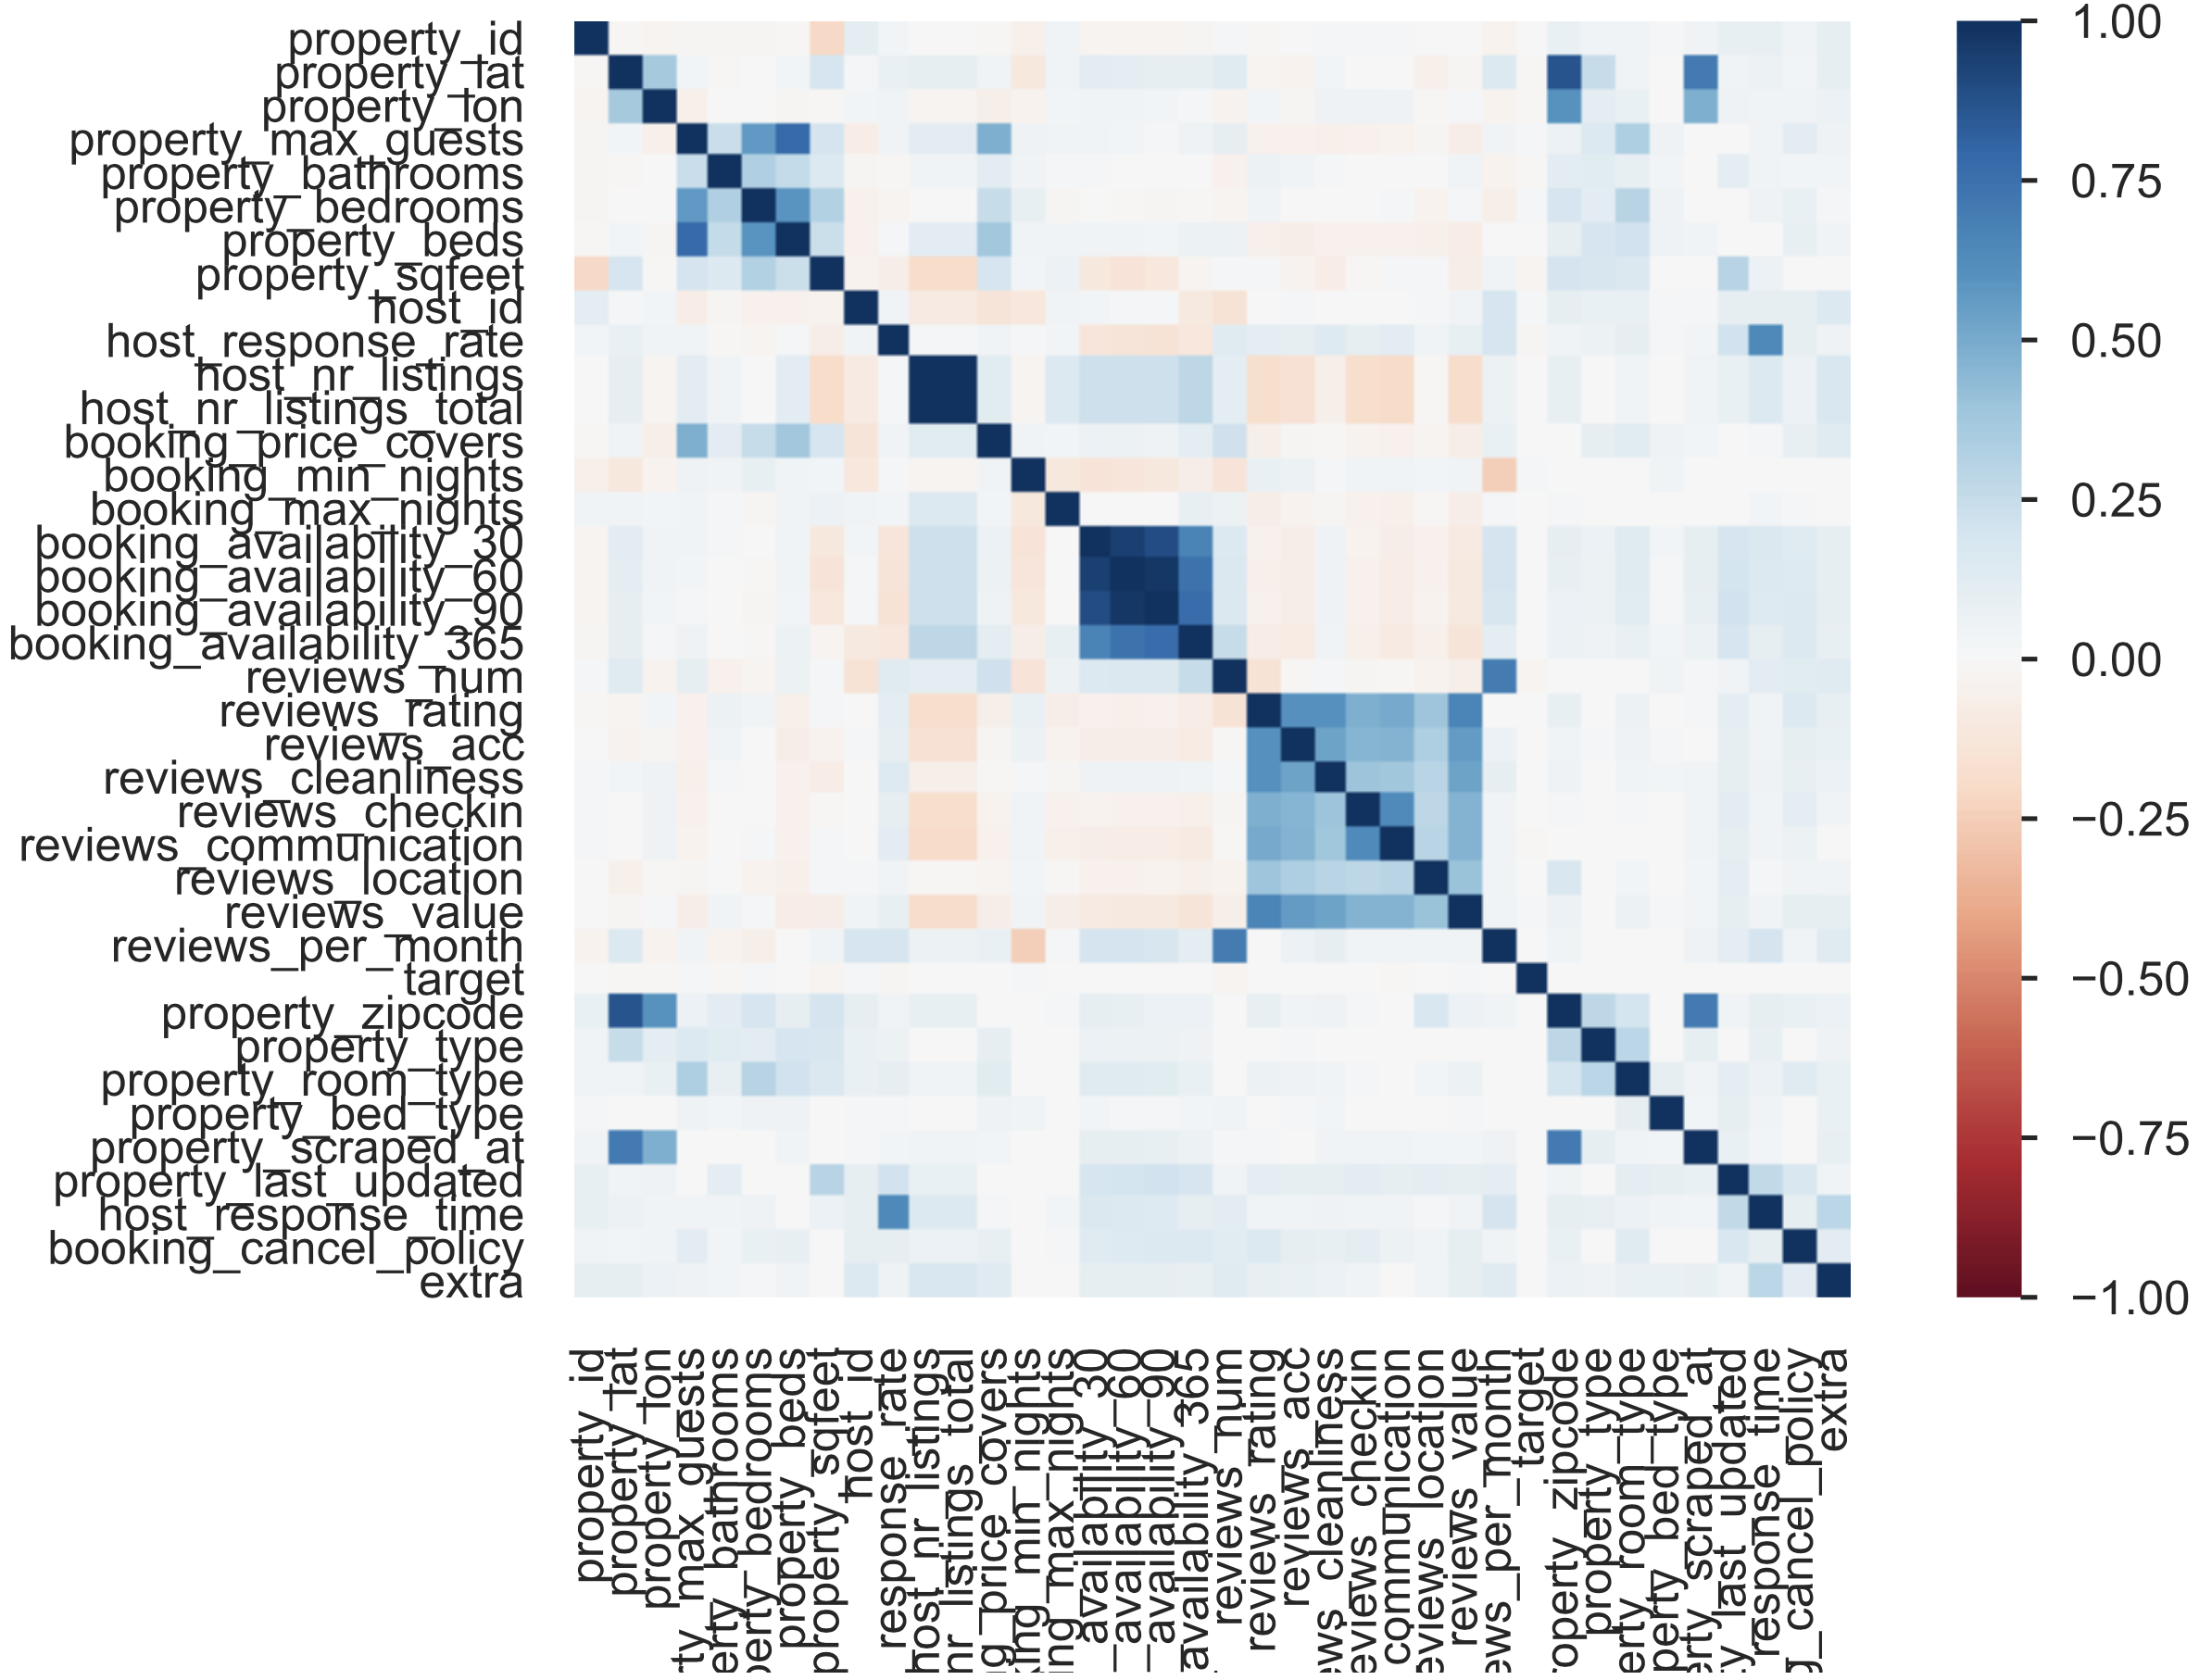
\includegraphics[width=1\linewidth]{Assignment1CorrInit}
\caption{Correlation heatmap of all original features}
\label{figure label}

	\centering
	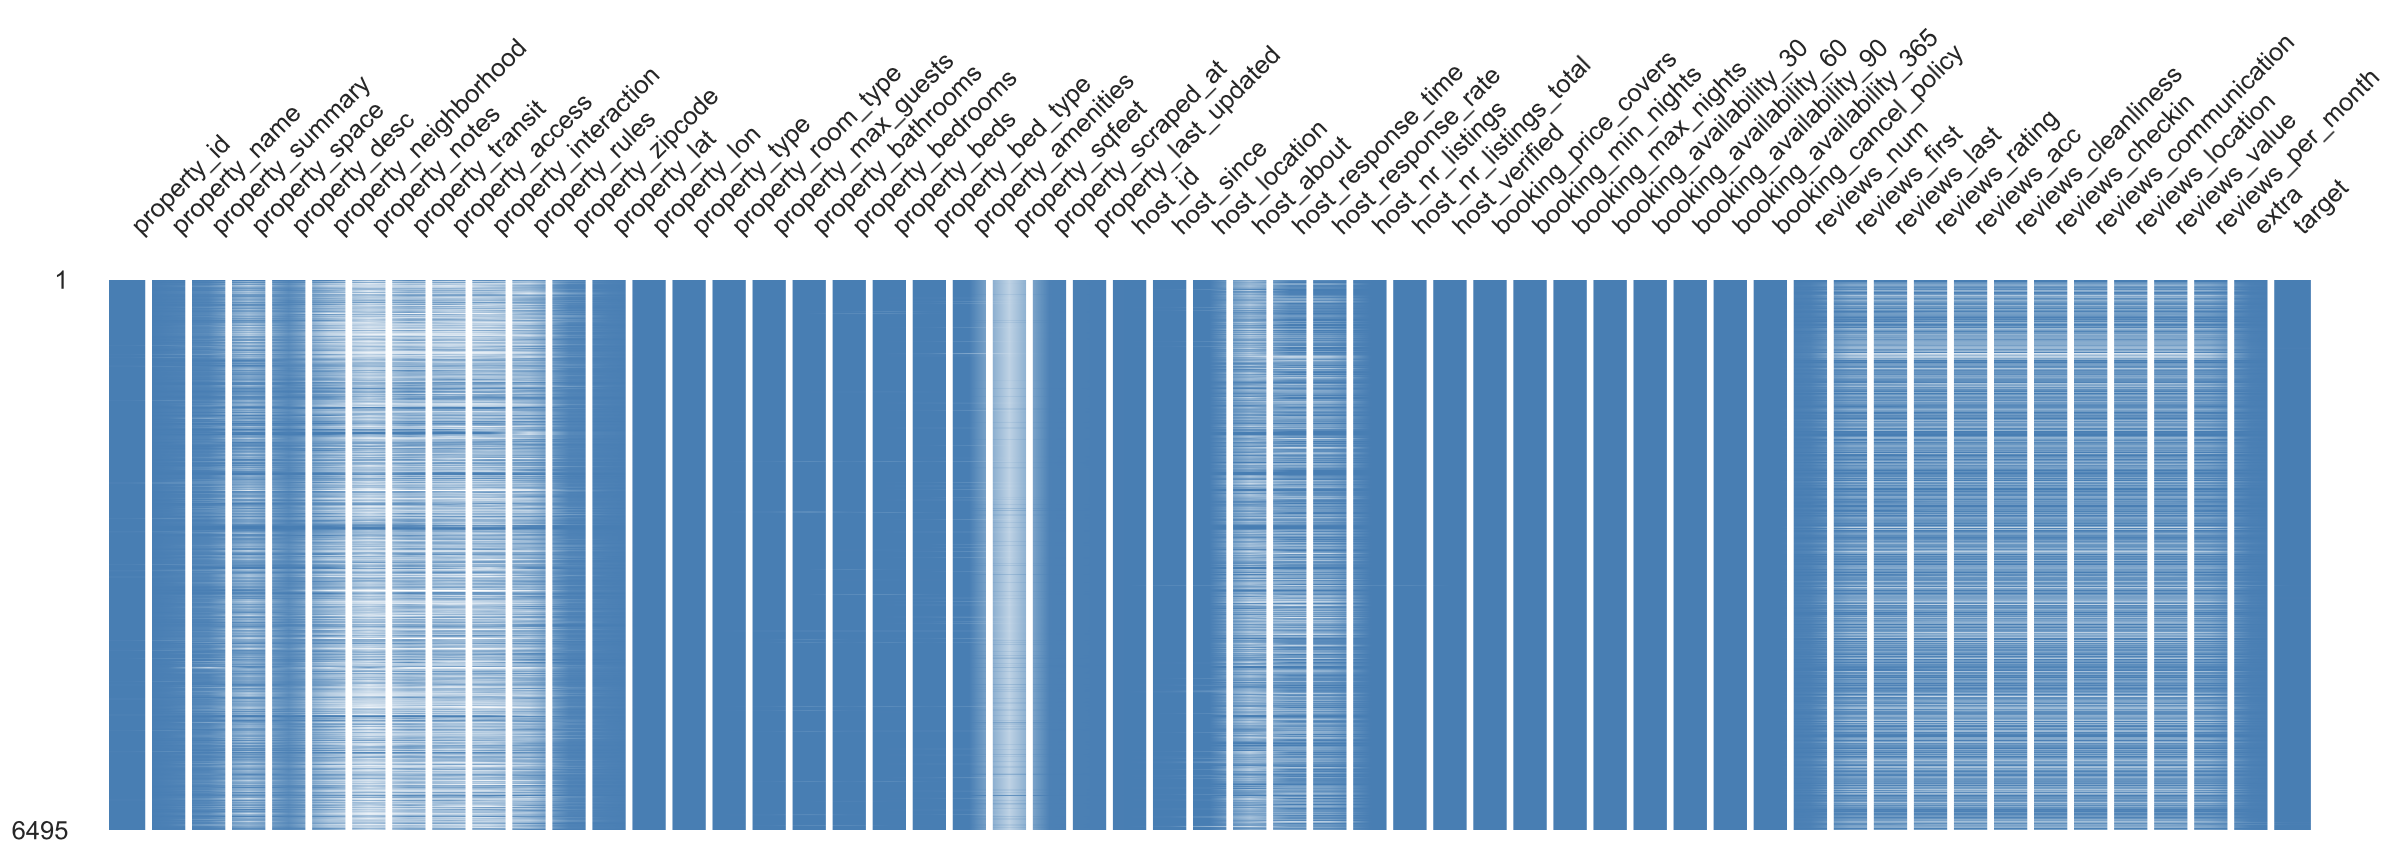
\includegraphics[width=1\linewidth]{NullityMatrix}
\caption{Nullity Matrix of all original features}
\label{figure label}
\end{figure}

\clearpage
\section{Predictive Model}
RandomForest, XGBoost and Linear Regression are tested as potential model candidates. Linear regression is left in the dust immediately and not further considered. RandomForest almost achieves parity with \textit{XGBoost} but always ever so slightly lags behind. Thus the clear method of choice remains \textit{XGBoost}.
\newline
\indent As a baseline score for orientation we calculated the mean (67.9) of the entire dataset and used it as a single-value predictor. The corresponding RMSE value on the test-set is $46.718$ and the Mean Average Error (MAE) is $28.138$. Throughout the process of trying out various models and manipulating the data back and forth, both scores proved elusive and difficult to reach, indicating there is generally little predictive power in the dataset. \newline
After fine-tuning \textit{XGBoost} on our validation-set, we settled on a maximum-tree-depth of 3, a subsampling-ratio of 0.8, a minimum-child-weight of 5 and a learning-rate/step-size shrinkage of 0.02.\newline
\indent Below table summarizes various scores for the validation- and test-set. Our model corresponds to \textit{tuned XGBoost}.
The test-metrics table indicates both the normal and the \textit{hidden} score, reflecting two separate test-sets of which only one was visible during model construction.
\newline
\begin{center}
\begin{tabular}{c | c c}
\textit{validation-metrics}&RMSE&MAE \\
\hline
tuned XGBoost&45.434&28.353\\
mean&45.435&28.855\\
randomForest&45.680&30.021\\
untuned XGBoost&57.138&33.0631
\end{tabular}
\end{center}

\begin{center}
\begin{tabular}{c | c c}
\textit{test-metrics}&RMSE&MAE \\
\hline
mean&46.718&28.138\\
tuned XGBoost&47.045&27.523\\
hidden mean&58.89&31.344\\
hidden tuned XGBoost&59.328&30.687
\end{tabular}
\end{center}
\section{Conclusion}
From above table it becomes clear the best "model" in terms of predictive performance is the arithmetic mean, once again highlighting the likely possibility the data holds vanishingly little predictive power.
\newline
\indent Furthermore, it is evident there are extreme values in the test-set as the RMSE value of our model is larger than that of the mean-predictor while our MAE value is smaller than that of the mean-predictor. This indicates our model has some marginal explanatory power but only manages to capture the presence of extreme observations insufficiently well. On our validation-dataset, however, our model manages to slightly outperform the mean-predictor (albeit after fine-tuning the model based on the validation-set, thereby incorporating it in our training-set to an extent).\newline
\indent A maximum tree-depth of 3 is prohibitive in the sense that only relatively coarse classification is possible. That this depth is the optimum in our case is another indication the data does not hold much predictive power. Figure 3 plots our predictions against the real-values of the validation set. The plot also shows the extent to which the data is beset with extreme values, i.e. listings with very high or low target prices.\newline
Overall, building a predictive model based on the data at hand proved astoundingly difficult. Despite various reconfigurations, our model could not convincingly beat the arithmetic mean.




\begin{figure}[h]

\centering
	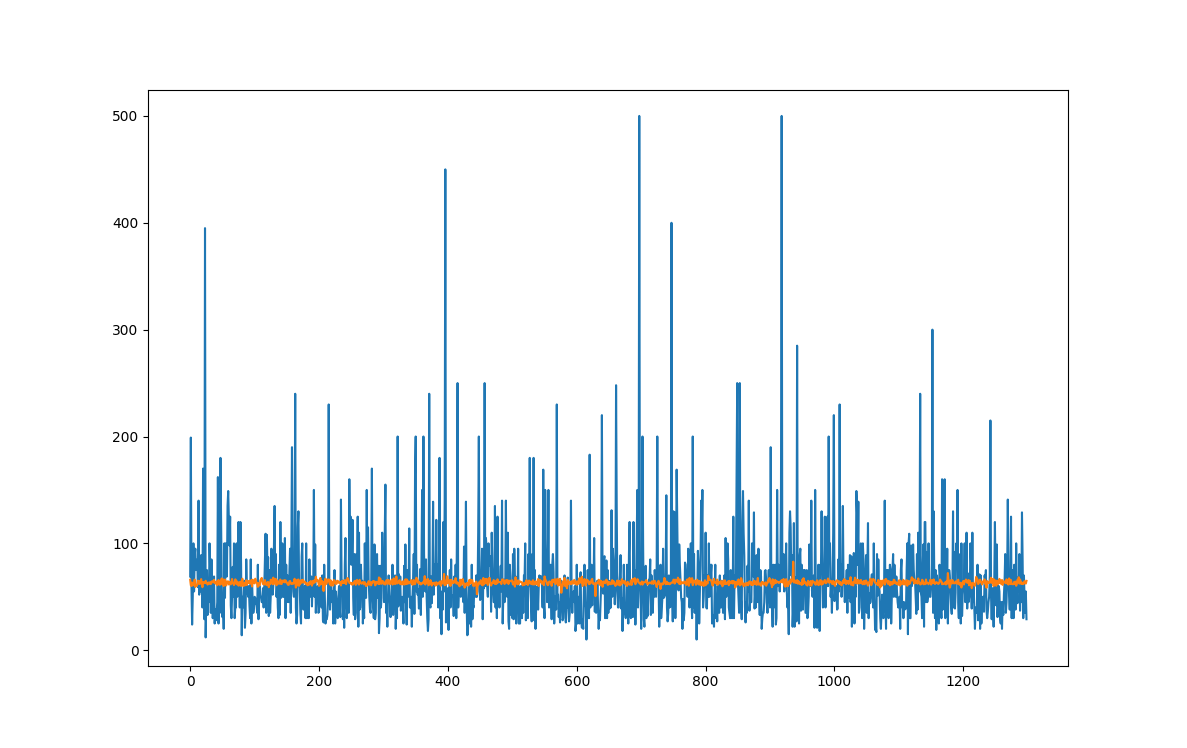
\includegraphics[width=1\linewidth]{PredsVSValids}
\caption{Plot of predicted values (orange) and targets (blue) on validation set}
\label{figure label}
\end{figure}

\begin{figure}[h!]
\centering
	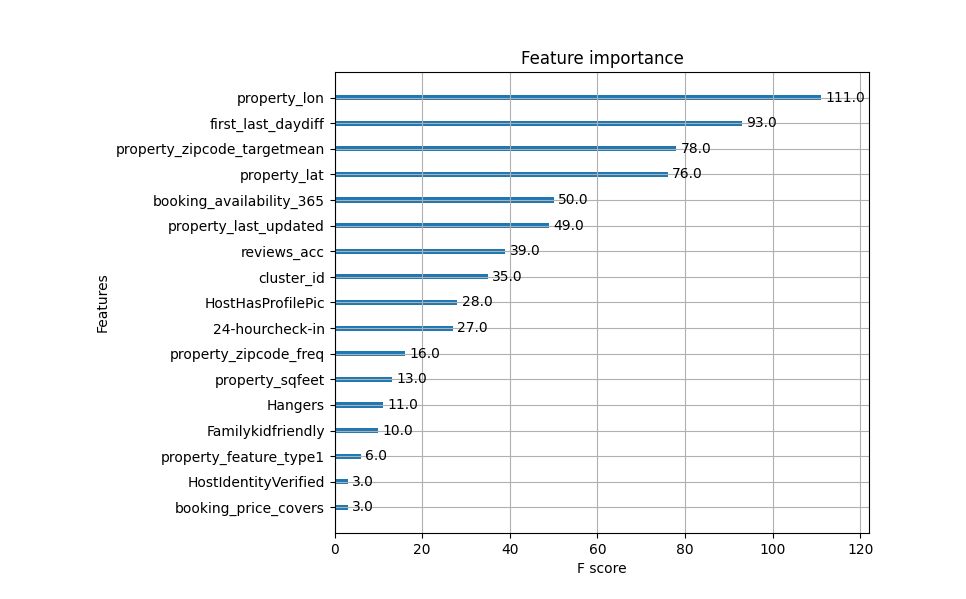
\includegraphics[width=1\linewidth]{FI_final}
\caption{Feature importance as calculated by the number of times a variable was split on}
\label{figure label}

\end{figure}


\end{document}  